\section{Single Photon Emitters}
\label{sec:SPE}
%Bei höheren Intensitäten sollte der Dip schmaler werde, weil dann der Emitter näher an Sättigung geht und zunehmend die Lebensdauer des angeregten Zustands statt der Einstrahlphotonenrate relevant ist
%Bei 2mW angefangen zu blinken. Spektrum trotzdem gut
%Für die Spektren gegen Wellenlänge die Fläche drunter integrieren und gegen Leistung plotten

\subsection{Execution}

Hexagonal boron nitride powder on a substrate is viewed through a confocal microscope, which is shown in \cref{fig_confocal}.
In order to navigate on the sample, a white light source and a camera are used.
Once a promising region is found, the laser is used instead and the detector (a spectrometer) is used, to record spectra at different spots on the sample, until a single photon emitter (SPE) is found.
The SPE is identified throught %TODO irgendwie, dass das Spektrum auf bestimmte Weise aussieht.


\begin{figure}[!ht]
    \centering
    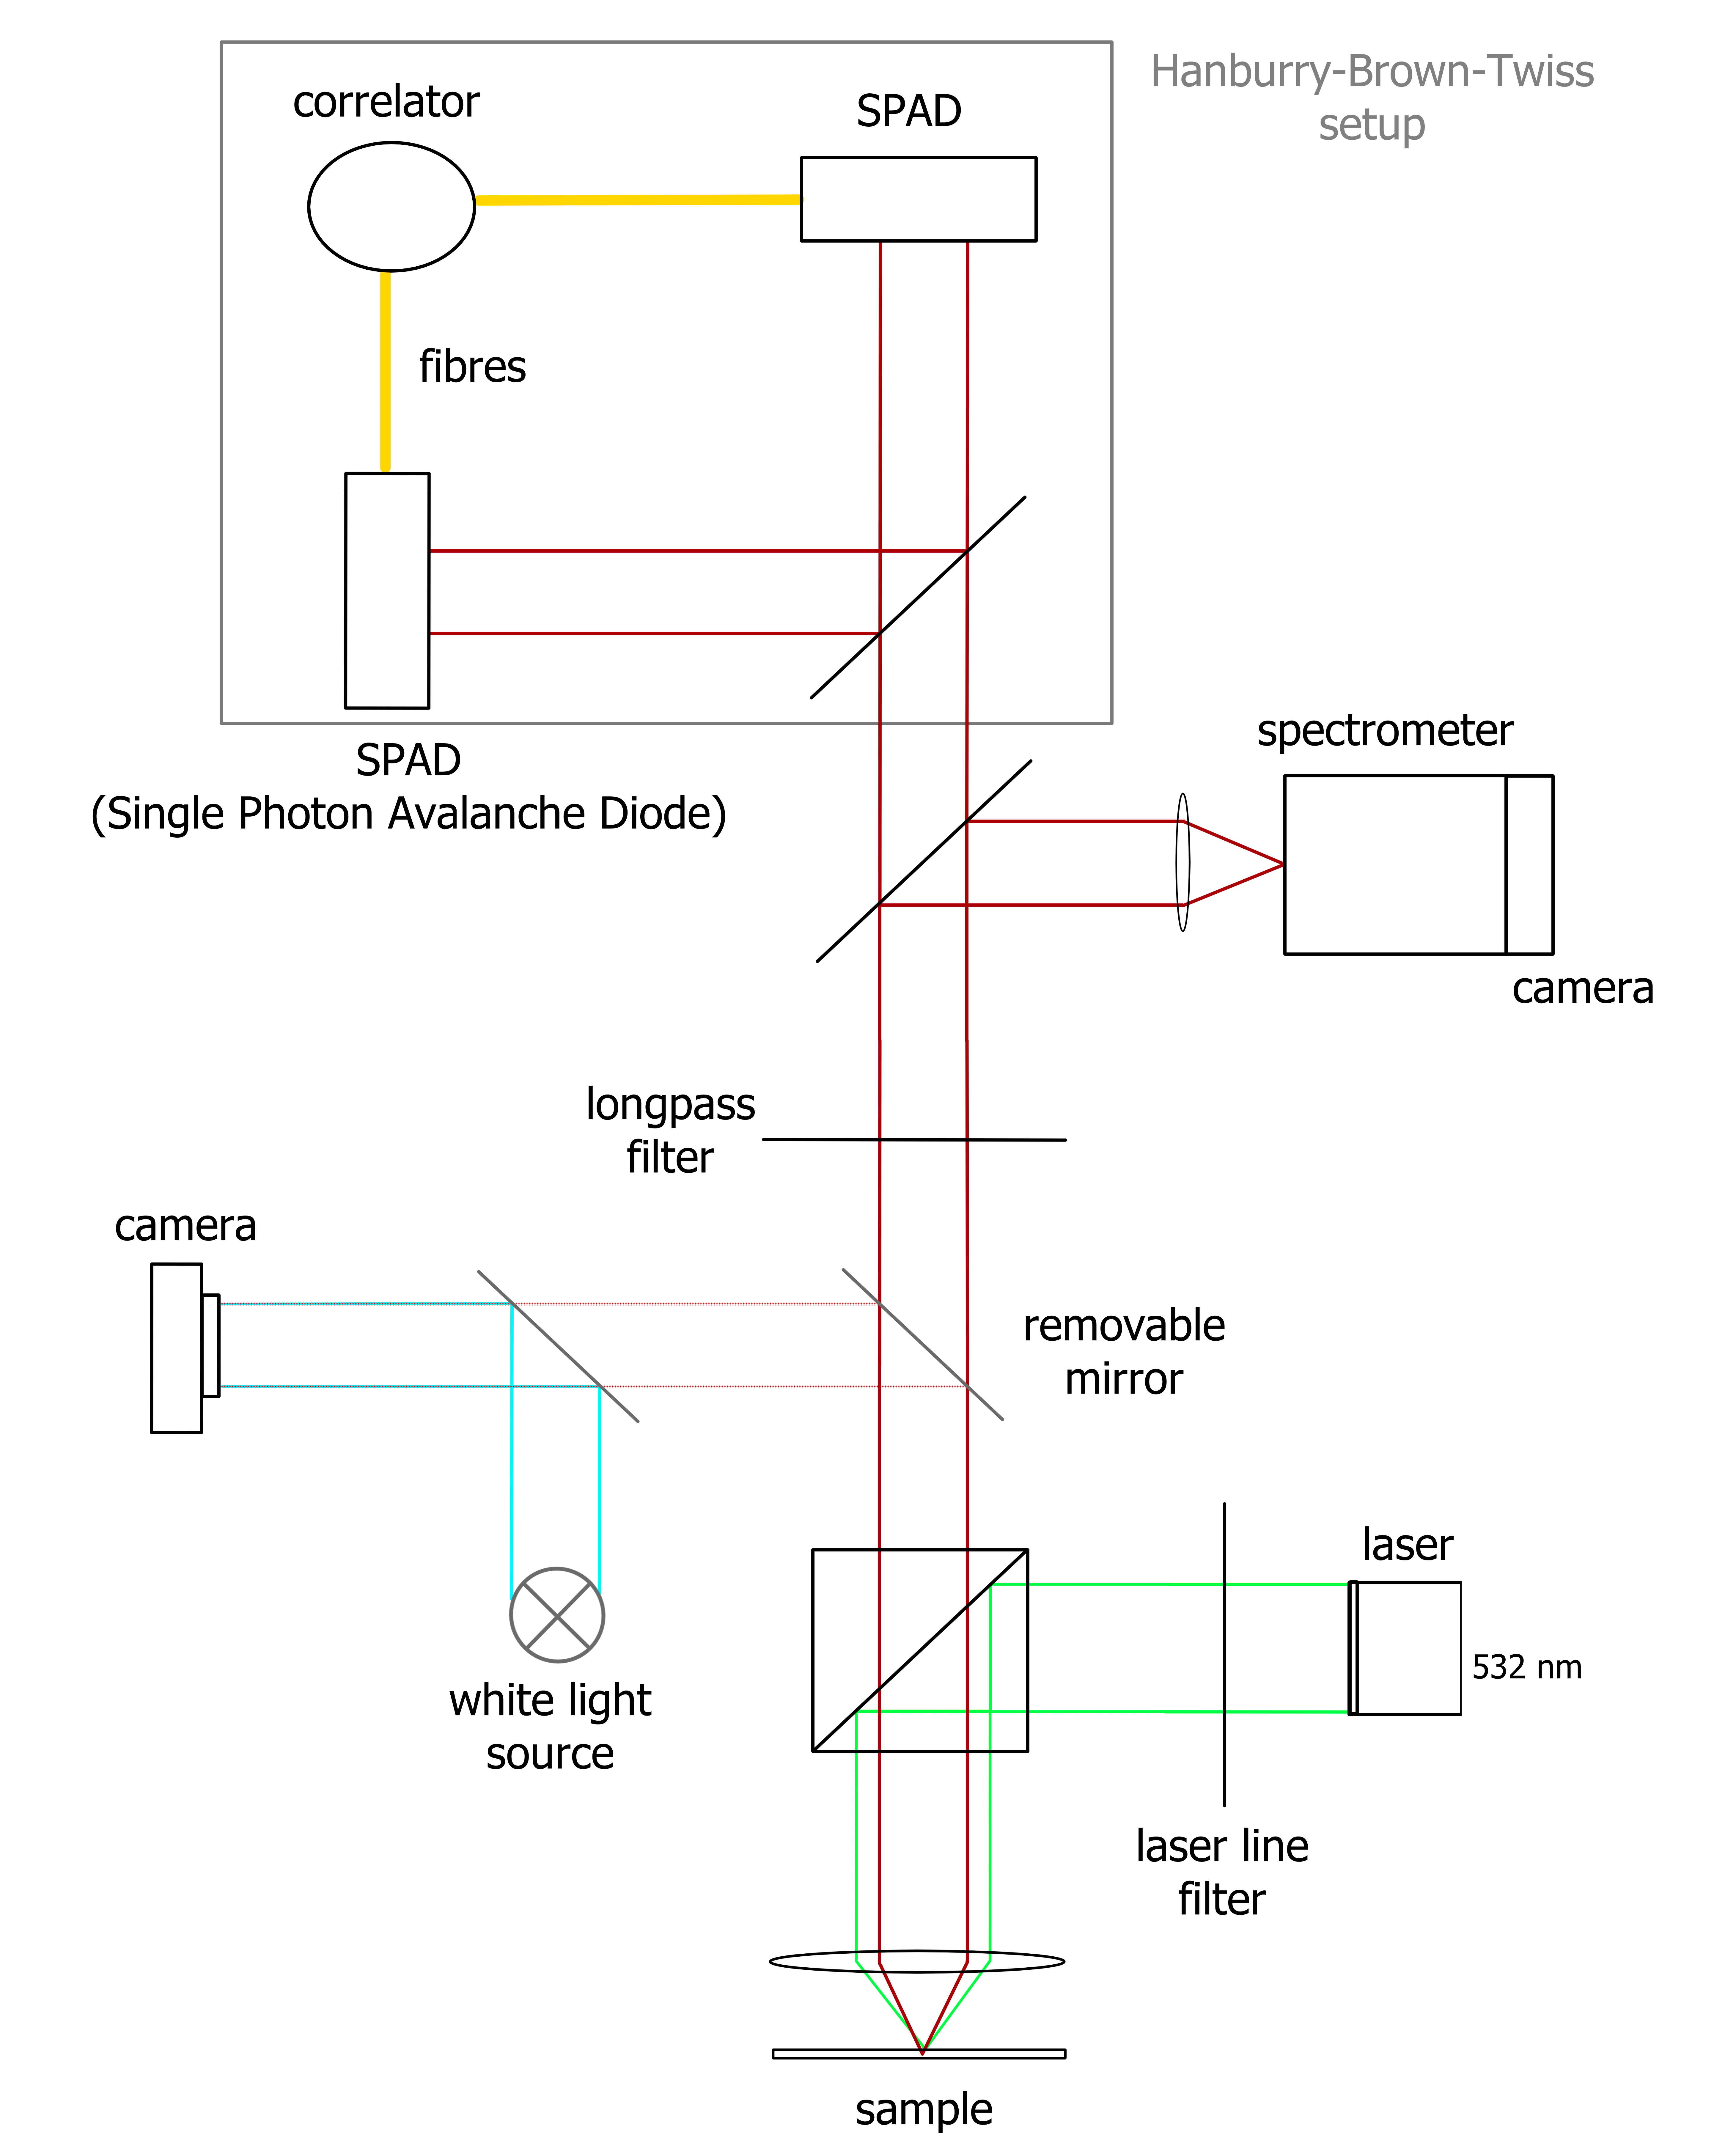
\includegraphics[width=0.7\textwidth]{img/setup2.png}
    \caption{Schematic of the confocal microscope used to record photoluminescence antibunching autocorrelation plots.}
    \label{fig_confocal}
\end{figure}

\subsection{Analysis}
